\begin{frame}{Catalyst sample: Pt nanoparticles}
    \medskip
    \begin{columns}

        \column[T]{0.45\textwidth}
    
            Patterned sample:
            \begin{itemize}
                \item Dewetted (111)-oriented nanoparticles
                \item (001)-oriented sapphire ($\alpha$-\ce{Al_2O_3}) substrate
                \item 24 hours annealed in air @1100°C
                %\item Model catalyst, similar to Pt foils
                % Wickham, D.T., B.A. Banse, and B.E. Koel, The adsorption of nitric oxide and nitrogen dioxide on polycrystalline platinum. Surf. Sci., 1989. 223: p. 82-100.
            \end{itemize}

            \vspace{0.5cm}
            \begin{figure}
                \centering
                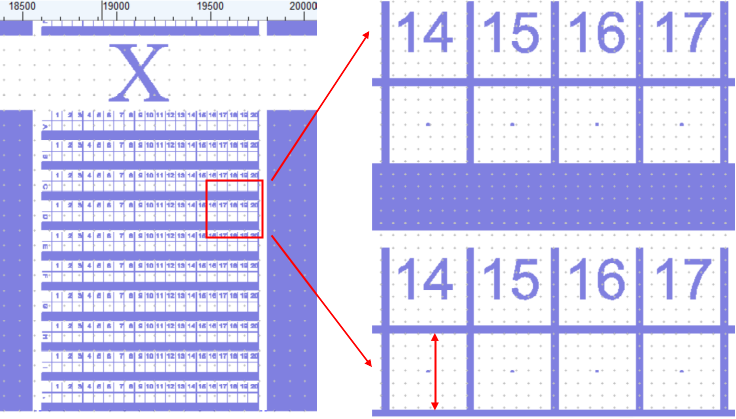
\includegraphics[width=\textwidth]{Figures/sample/mask.png}
                \caption{Mask during sample preparation (area in blue)}
                \label{fig:mask}
            \end{figure}

        \pause
        \column[T]{0.5\textwidth}

            \begin{figure}
                \centering %left bottom right top
                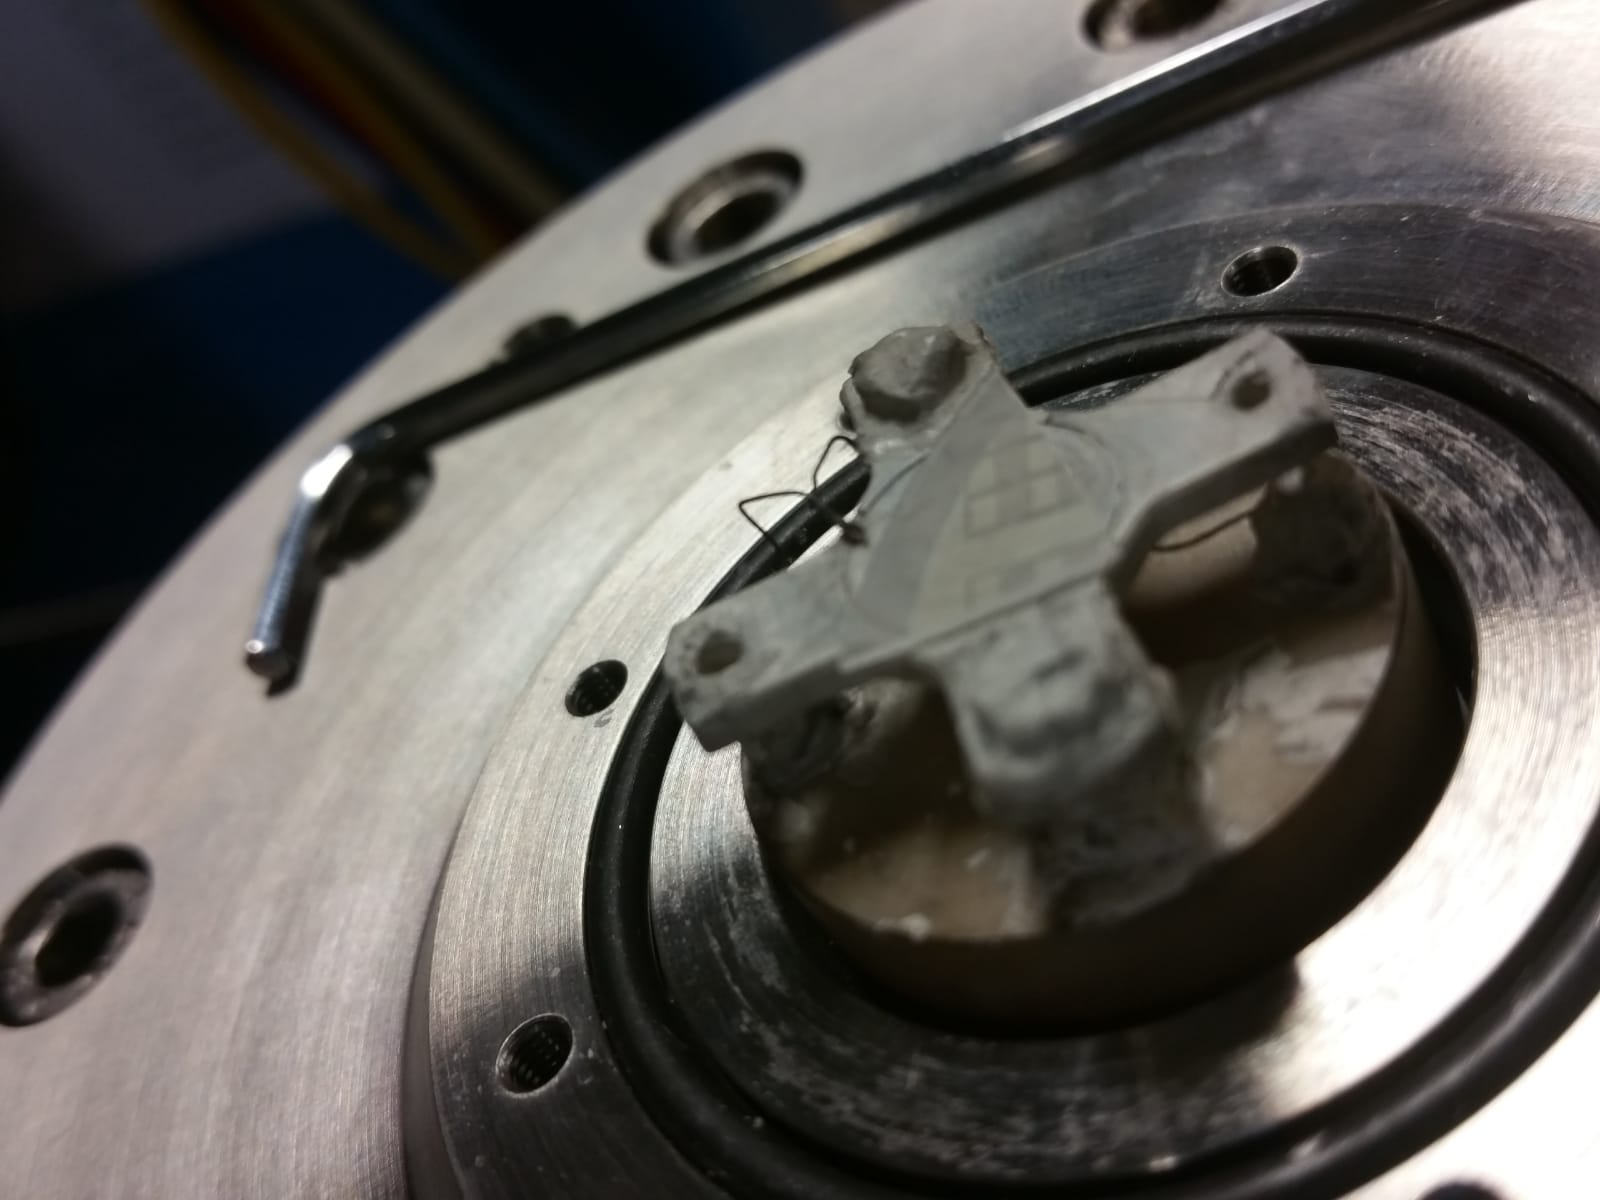
\includegraphics[trim=650 300 250 250, clip, width=0.45\textwidth]{Figures/sample/reactor_cell.jpeg}
                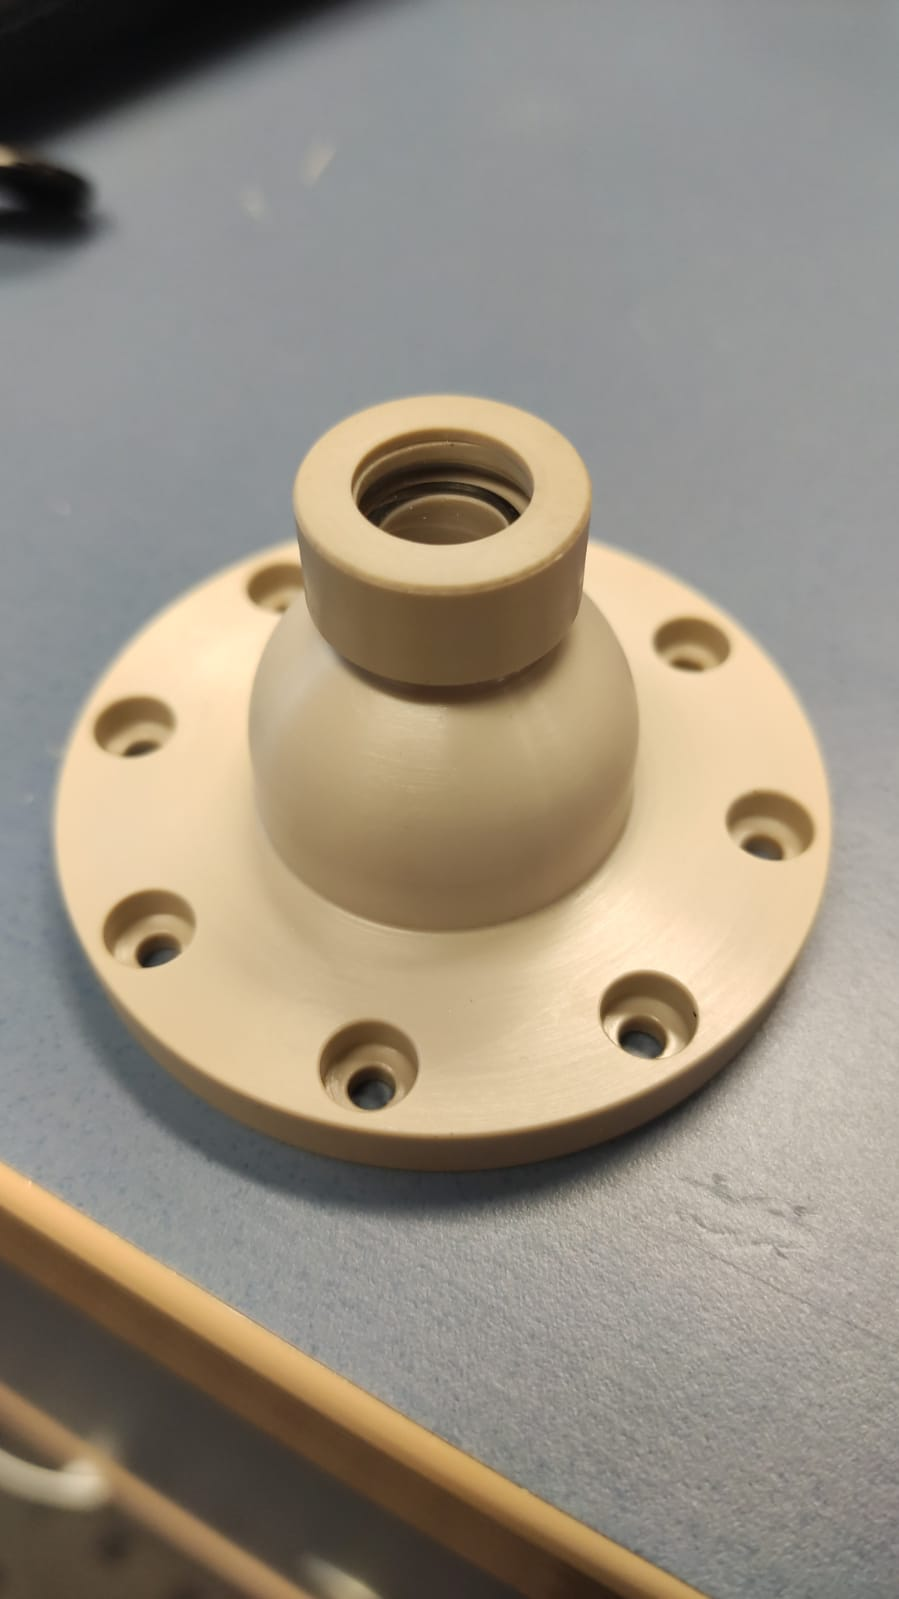
\includegraphics[trim=0 400 0 380, clip, width=0.45\textwidth]{Figures/sixs/dome_window.png}
                \caption{Sample holder, paste in Boron Nitride, wafer in Sapphire.}
                \label{fig:sample_and_dome}
            \end{figure}

            \pause
            
            \begin{figure}
                \centering %left bottom right top
                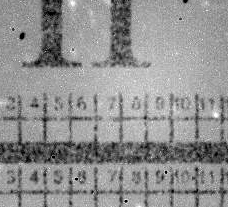
\includegraphics[trim=0 0 0 10, clip, width=0.45\textwidth]{Figures/sample/microscope_image.png}
                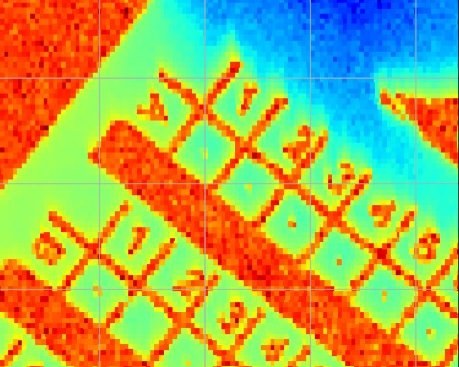
\includegraphics[width=0.45\textwidth]{Figures/sample/microscope_image_photon.png}
                \caption{Microscope image}
                \label{fig:microscope_image}
            \end{figure}
    \end{columns}

\end{frame}